The last trick for our bag to embark on the KFAC journey is linearization.
It is a useful tool whenever we encounter a composition of functions that we would like to convexify.

\paragraph{Convexification by partial linearization.}
Consider \eg the function $f = g \circ h$ with $f,g,h: \sR \to \sR$ for simplicity.
We know that convexity is preserved under function composition, so if both $g$ and $h$ are convex, then $f$ will be convex.
But what if only one of the two composites is convex, lets say $g$, but $h$ is not?
Well, then we can replace $h$ with an approximation $h'$ that is convex and approximates the original function.
One straightforward approximation is a linear approximation.

\paragraph{Linearization.} Let's say we are interested in only a neighbourhood around $x_0$.
Then, we can obtain a simple, convexified approximation $\bar{f} \approx f$ in that neighbourhood by linearizing $h$ around $x_0$, resulting in a function $(\lin_{x_0}(h))(x)$.
This involves a first-order Taylor approximation:

\begin{definition}[Linearization (vector case, \Cref{basics/linearization})]\label{def:vector_linearization}
  Consider a vector-to-vector function $f$ from \Cref{setup:vector_to_vector_function}.
  The linearization of $f$ at an anchor point $\va_0 \in \sR^A$ denoted by $\lin_{\va_0}(f): \sR^A \to \sR^B$ is its first-order Taylor expansion,
  \begin{align*}
    (\lin_{\va_0}(f))(\va) = f(\va_0) + \jac_{\va_0}f(\va_0) (\va - \va_0)
  \end{align*}
  with the Jacobian from \Cref{def:vector_jacobian}.
  Note that $\lin_{\va_0}(f)$ is linear in $\va$ and coincides with the original function at the anchor point, $(\lin_{\va_0}(f))(\va_0) = f(\va_0)$.
  Its Jacobian also concides with that of the original function at the anchor point.
\end{definition}

The generalization to the tensor case is straightforward.
We just need to replace the Jacobian-vector product with its generalization:

\switchcolumn[1]
\codeblock{basics/linearization}
\switchcolumn[0]

\begin{definition}[Linearization (tensor case, \Cref{basics/linearization})]\label{def:tensor_linearization}
  The linearization of a tensor-to-tensor function from \Cref{setup:jacobians} at an anchor point $\tA_0 \in \sR^{A_1 \times \ldots \times A_N}$, denoted by $\lin_{\tA_0}(f)$ is defined per-entry as
  \begin{align*}
    & \left[
      (\lin_{\tA_0}(f))(\tA)
      \right]_{i_1, \ldots, i_M} = f(\tA_0)
    \\
    & \hspace{2em}+
      \sum_{j_1, \ldots, j_N}
      \left[
      \jac_{\tA_0}f(\tA_0)
      \right]_{i_1, \ldots, i_M, j_1, \ldots, j_N}
    \\
    & \hspace{6.2em}\left[
      \tA - \tA_0
      \right]_{j_1, \ldots, j_N}\,,
  \end{align*}
  with the Jacobian from \Cref{def:general_jacobian}. Note that this is nothing else but the function evaluated at the anchor point plus the JVP (\Cref{def:jvp}) with the distance to the anchor.
\end{definition}

\paragraph{GGN \& relevance to deep learning.}
In deep learning, we will often face the situation where $f = g \circ h, \tA \mapsto b = f(\tA)$ and $h$ is non-convex while $g$ is convex
(\eg in the empirical risk, where the criterion is typically convex, while the neural net is typically non-convex).
This means the Hessian of $f$ can be indefinite; but many algorithms require a positive definite approximation to the Hessian.
We can obtain that by considering the partially linearized function $\bar{f} = g \circ \lin_{\tA_0}(h)$, whose Hessian is positive semi-definite.
The Hessian of this partially linearized function is called the generalized Gauss-Newton (GGN) matrix.

Let's stick to our one-dimensional example for a moment, \ie let $f(x) = (g \circ h)(x) \in \sR$.
If we use the chain rule twice, we obtain $f'' = g' h'' g' + h' g''$ for the second derivative. Using our Jacobian and Hessian notation, this translates into
\begin{align*}
  &\hess_x f(x)
  \\
  &=\hess_x (g \circ h)(x)
  \\
  &=\jac_x h(x) \cdot \hess_{h(x)} g(h(x)) \cdot \jac_x h(x)
  \\
  &\phantom{= }+
    \hess_x h(x) \cdot \jac_{h(x)} g(h(x))\,.
\end{align*}
Now, if we take the Hessian of the partially linearized function $\bar{f}(x) = (g \circ \lin_{x_0}(h))(x)$, and use the shorthand $\bar{h} = \lin_{x_0}(h)$ the second term disappears as the linear function's Hessian is zero:
\begin{align*}
  &\hess_x \bar{f}(x)
  \\
  &=\hess_x (g \circ \bar{h})(x)
  \\
  &=\jac_x \bar{h}(x) \cdot \hess_{\bar{h}(x)} g(\bar{h}(x)) \cdot \jac_x \bar{h}(x)
  \\
  &\phantom{= }+
    \underbrace{\hess_x \bar{h}(x)}_{= 0} \cdot \jac_{\bar{h}(x)} g(\bar{h}(x))\,.
\end{align*}
Evaluating both equations at the anchor point (setting $x = x_0$) we see that their first terms coincide (remember from \Cref{def:vector_linearization} that the linearized function's value and Jacobian coincide with those of the original function when evaluated at the anchor point).

\switchcolumn[1]*
\begin{figure}[!h]
  \centering
  \begin{tikzpicture}[%
    font=\scriptsize,%
    thick,
    box/.style = {rectangle, draw=black, rounded corners, fill=VectorGray!50},%%
    ]
    \node[box] (A) at (0,0) {$f = g \circ h: \tA \mapsto \tB \mapsto c$};
    \node[box] (B) at (5.5,0) {$\tH_{\tA}c$};
    \node[box, align=center] (C) at (0,-3) {%
      $\bar{f}_{\tA_0} = g \circ \lin_{\tA_0} h$\\%
    };
    \node[box, align=center] (D) at (5.5,-3) {%
      $\tG_{\tA}f(\tA)|_{\tA = \tA_0}$
      \\
      $=$\\%
      $\tH_{\tA} \bar{f}_{\tA_0}(\tA)|_{\tA = \tA_0}$\\%
    };
    \draw[-Stealth] (A.east) -- node[fill=white] {$\tH$} (B.west);
    \draw[-Stealth] (A.south) -- node[fill=white, align=center] {partially linearize $h$ \\
      around some $\tA_0$} (C.north);
    \draw[-Stealth] (C.east) -- node[fill=white, align=center] {$\tH$, then\\ set\\ $\tA_0 = \tA$} (D.west);
    \draw[-Stealth] (B.south) -- node[fill=white, align=center] {ignore second-order\\ effects of $h$} (D.north);
  \end{tikzpicture}
  \caption{\textbf{Taking the Hessian and partial linearization commute and lead to the same GGN.}
    All operations also commute with flattening the function versus matrizicing the Hessian tensor, so we can apply any flattening scheme on top to obtain the $\rvec$- and $\cvec$-GGN matrices.}\label{fig:commutative-diagram-ggn}
\end{figure}
\switchcolumn[0]

Hence, our one-dimensional example's GGN is
\begin{align*}
  &G_{x_0} f(x_0)
  \\
  &=\jac_{x_0} h(x_0) \cdot \hess_{h(x_0)} g(h(x_0)) \cdot \jac_{x_0} h(x_0)\,.
\end{align*}
To summarize, we obtain the GGN either by (i) partially linearizing, then taking the Hessian, or (ii) taking the Hessian and discarding second-order derivatives of the non-convex composite (\ie partially linearizing).
This commutative relationship is visualized in \Cref{fig:commutative-diagram-ggn}.
Our next steps are to generalize the GGN to vector-valued functions that produce scalars, illustrate it on a toy problem, then develop the fully general formulation for tensor-valued functions along with the functionality to work with it in code.

\switchcolumn[1]*
\begin{figure}[H]
  \centering
  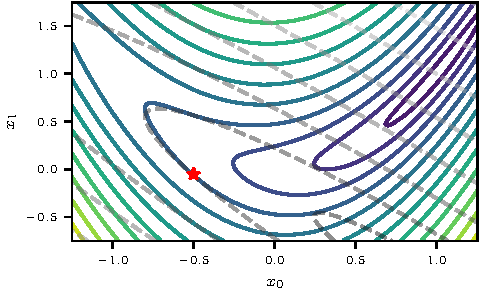
\includegraphics[width=\linewidth]{../kfs/plots/linearized_rosenbrock.pdf}
  \caption{\textbf{The 2d Rosenbrock function} $f_{\alpha=10}$ (solid contour lines) and its convex approximation $\bar{f}_{\alpha=10} = g \circ \bar{h}_{\alpha=10}$ (dashed contour lines) around an anchor $\hat{\vx}$ (star) from partial linearization.
    The convex approximation is a quadratic form with the GGN.}\label{fig:2d-rosenbrock}
\end{figure}
\switchcolumn[0]

\paragraph{Vector case with basic example.}
We already introduced notation for the GGN.
Let's define it for the vector case and apply it to an example.

\switchcolumn[1]
\codeblock{basics/ggn_rosenbrock}
\switchcolumn[0]

\begin{setup}[Composite vector-to-vector-to-scalar function]\label{setup:composite_vector_to_vector_to_scalar_function}
  Let
  \begin{align*}
    f: \sR^{A} & \to \sR
    \\
    \va        & \mapsto c = f(\va)
  \end{align*}
  be the composite of a vector-to-vector function $h$ and a vector-to-scalar function $g$, that is
  \begin{align*}
    f = g \circ h: \sR^A & \to \sR^B \to \sR
    \\
    \va                  & \mapsto \vb = h(\va) \mapsto c = g(\vb)\,.
  \end{align*}
\end{setup}

\begin{definition}[GGN matrix (vector case)]\label{def:vector_ggn}
  The GGN matrix of a vector-to-vector-to-scalar function $f$ from \Cref{setup:composite_vector_to_vector_to_scalar_function} is
  \begin{align*}
    \ggn_{\va} f(\va)
    =
    (\jac_{\va} \vb)^{\top}
    (\hess_{\vb} c)
    (\jac_{\va} \vb) \in \sR^{A \times A}\,,
  \end{align*}
  \ie the second composite's Hessian, pulled back with the first composite's Jacobian.
\end{definition}

One obtains this form by following through the same steps as above, but for a vector-to-vector-to-scalar instead of a purely scalar function composition. \Cref{ex:ggn-rosenbrock} presents fully-worked out expressions of Rosenbrock function's GGN.

\begin{example}[GGN for the Rosenbrock function, \Cref{basics/ggn_rosenbrock}]\label{ex:ggn-rosenbrock}
  Consider the 2d Rosenbrock function $f_{\alpha}: \sR^2 \to \sR$ with
  \begin{align*}
    f_{\alpha}(\vx)
    =
    (1 - x_1)^2 + \alpha (x_2 - x_1^2)^2\,.
  \end{align*}
  with some $\alpha > 0$.

  \paragraph{Composition.}
  Following \citet{brunet2010basics}, we express the Rosenbrock function as vector-to-vector-to-scalar function
  \begin{align*}
    f_{\alpha} &= g \circ h_{\alpha}: \sR^2 \to \sR^2 \to \sR
                 \shortintertext{with}
                 h_{\alpha}(\vx) &= \begin{pmatrix}
                   1 - x_1 \\
                   \sqrt{\alpha} (x_2 - x_1^2)
                 \end{pmatrix}
                                   \shortintertext{and convex}
                                   g(\vh) &= \vh^\top \vh\,,
  \end{align*}
  namely square loss.

  \paragraph{Linearization.}
  The Rosenbrock function is non-convex (see \Cref{fig:2d-rosenbrock} for contour lines) because $h_{\alpha}$ is non-convex.
  We want to convexify it by partial linearization.
  Linearizing $h_{\alpha}$ \wrt $\vx$ around an anchor $\hat{\vx}$ gives
  \begin{align*}
    \bar{h}_{\alpha}(\vx)
    &=
      h_{\alpha}(\hat{\vx}) + (\jac_{\hat{\vx}}h_{\alpha}(\hat{\vx})) (\vx - \hat{\vx})
      \shortintertext{with the Jacobian}
      \jac_{\vx}h_{\alpha}(\vx)
    &=
      \begin{pmatrix}
        -1                   & 0             \\
        -2 \sqrt{\alpha} x_1 & \sqrt{\alpha}
      \end{pmatrix}\,.
  \end{align*}
  Inserting all expressions, we have
  \begin{align*}
    \bar{h}_{\alpha}(\vx)
    =
    \begin{pmatrix}
      1 - \hat{x}_1 \\
      \sqrt{\alpha} (\hat{x}_2 - \hat{x}_1^2)
    \end{pmatrix}
    \\
    +
    \begin{pmatrix}
      \hat{x}_1 - x_1 \\
      2 \sqrt{\alpha} \hat{x}_1 (\hat{x}_1 - x_1) + \sqrt{\alpha} (x_2 - \hat{x}_2)
    \end{pmatrix}
    \\
    =
    \begin{pmatrix}
      1 - x_1
      \\
      2 \sqrt{\alpha} \hat{x}_1 \left( \frac{1}{2} \hat{x}_1 - x_1 \right) +  \sqrt{\alpha} x_2
    \end{pmatrix}
  \end{align*}
  Note that this function is indeed linear in $x_{1,2}$.

  \paragraph{Partial linearization.}
  With $\bar{h}_{\alpha}(\vx)$, we can evaluate the partially linearized Rosenbrock function $\bar{f}_{\alpha} = g \circ \bar{h}_{\alpha}$ as
  \begin{align*}
    \bar{f}_{\alpha}(\vx)
    &=
      (\bar{h}_{\alpha}(\vx))^{\top} \bar{h}_{\alpha}(\vx)
    \\
    &=
      (1 - x_1)^2
    \\
    &\phantom{= }+
      \alpha \left[ 2 \hat{x}_1 \left(\frac{1}{2} \hat{x}_1 - x_1 \right) +  x_2 \right]^2
    \\
    &= 1 - 2x_1 + x_1^2 + \alpha [ 2 \hat{x}_1^4 - 4 \hat{x}_1^3 x_1
    \\
    &\phantom{= }+ 4 \hat{x}_1^2 x_1^2 - 2 \hat{x}_1^2 x_2 - 4 \hat{x}_1 x_1 x_2 + x_2^2 ]\,.
  \end{align*}

  \paragraph{GGN via linearize-then-differentiate.}
  The Rosenbrock's GGN is the Hessian of its partial linearization, evaluated at $\vx = \hat{\vx}$
  \begin{align*}
    \ggn_{\hat{\vx}} f_{\alpha}(\hat{\vx})
    &=
      \hess_{\vx} \bar{f}_{\alpha}(\vx)|_{\vx=\hat{\vx}}
    \\
    &=
      2
      \begin{pmatrix}
        1 + 4 \alpha \hat{x}_1^2 & - 2\alpha \hat{x}_1
        \\
        - 2\alpha \hat{x}_1 & \alpha
      \end{pmatrix}\,.
  \end{align*}

  \paragraph{GGN via differentiate-then-linearize.}
  Let's double-check our result by evaluating the GGN in \cref{def:vector_ggn}, which follows by differentiating twice, then neglecting non-linearities of $h_{\alpha}$,
  \begin{align*}
    \ggn_{\hat{\vx}} f_{\alpha}(\hat{\vx})
    =&
       (\jac_{\vx} h_{\alpha}(\vx) )^{\top}|_{\vx = \hat{\vx}}
    \\
     &\hess_{h_{\alpha}(\vx)} g(h_{\alpha}(\vx)) |_{h_{\alpha}(\vx) = h_{\alpha}(\hat{\vx})}
    \\
     &\jac_{\vx} h_{\alpha}(vx) |_{\vx = \hat{\vx}}\,.
       \shortintertext{Using the Rosenbrock's Jacobian from above, and the square loss Hessian from \Cref{ex:square_loss_hessian} which is proportional to the identity, yields}
       =&
          2
          (\jac_{\vx} h_{\alpha}(\vx) )^{\top}|_{\vx = \hat{\vx}}
    \\
     &
       \jac_{\vx} h_{\alpha}(\vx) |_{\vx = \hat{\vx}}
    \\
    =&
       2
       \begin{pmatrix}
         -1                   & -2 \sqrt{\alpha} x_1 \\
         0 & \sqrt{\alpha}
       \end{pmatrix}
    \\
     &
       \begin{pmatrix}
         -1                   & 0             \\
         -2 \sqrt{\alpha} x_1 & \sqrt{\alpha}
       \end{pmatrix}
    \\
    =&
       2
       \begin{pmatrix}
         1 + 4 \alpha \hat{x}_1^2 & - 2\alpha \hat{x}_1
         \\
         - 2\alpha \hat{x}_1 & \alpha
       \end{pmatrix}\,.
  \end{align*}
  This is the same expression we obtained with the linearize-then-differentiate approach.
 We also see that the GGN is positive semi-definite, as it is a scaled outer product of Jacobians.

 \paragraph{Comparison of Hessian and GGN.}
 As expected, the Rosenbrock function's Hessian, evaluated at $\hat{\vx}$, is different from the GGN:
  \begin{align*}
    &\hess_{\vx} f_{\alpha}(\vx)|_{\vx = \hat{\vx}}
      \\
    &=
    2
    \begin{pmatrix}
      1 + 6 \alpha \hat{x}_1^2 - 2 \alpha \hat{x}_2 & -2 \alpha \hat{x}_1 \\
      -2 \alpha \hat{x}_1                      & \alpha
    \end{pmatrix}\,.
  \end{align*}
\end{example}

\paragraph{Generalization to tensor case.} The above example illustrated the GGN for a vector-to-vector-to-scalar function.
We will spend the remaining part of this section to generalize the GGN to tensor-to-tensor-to-scalar functions.
Note that we already generalized all ingredients (linearization from \Cref{def:tensor_linearization}, the Jacobian tensor from \Cref{def:general_jacobian}, and the Hessian tensor from \Cref{def:general_hessian}) to that scenario.
All we have to do is put them together.
After that, we will see a tensor case example of the GGN that will be extremely relevant for our KFAC journey.

\switchcolumn[1]
\codeblock{basics/ggns}
\switchcolumn[0]

\begin{setup}[Composite tensor-to-tensor-to-scalar function]\label{setup:composite_tensor_to_tensor_to_scalar_function}
  Let the tensor-to-scalar map
  \begin{align*}
    f: \sR^{A_1 \times \ldots \times A_N} & \to \sR
    \\
    \tA                                   & \mapsto c = f(\tA)
  \end{align*}
  be the composite of a tensor-to-tensor function $h$ and a tensor-to-scalar function $g$, that is
  \begin{align*}
    f = g \circ h: & \sR^{A_1 \times \ldots \times A_N} \to \sR^{B_1 \times \ldots \times B_M}  \to \sR\!\!
    \\
                   & \tA \mapsto \tB = h(\tA) \mapsto c = g(\tB)\,.
  \end{align*}
\end{setup}

\begin{definition}[Generalized Gauss-Newton (GGN) tensor (\Cref{basics/ggns})]\label{def:general_ggn}%
  The GGN tensor of a tensor-to-tensor-to-scalar map $f$ from \Cref{setup:composite_tensor_to_tensor_to_scalar_function}, $\tG_{\tA} f(\tA) \in \sR^{A_1 \times \ldots \times A_N \times A_1 \times \ldots \times A_N}$ is the Hessian of the partially linearized function $\bar{f} = g \circ \lin_{\tA_0}(h)$, evaluated at the anchor point $\tA = \tA_0$.
  \begin{align*}
    \tG_{\tA} f(\tA)
    =
    \tH_{\tA} \bar{f}(\tA)|_{\tA = \tA_0}\,.
  \end{align*}
  where $\bar{f} = g \circ \lin_{\tA_0}(h)$.

  Similar to the vector case (\Cref{def:vector_ggn}), we can express this tensor as a contraction between the Jacobians and Hessians of the two composites, \ie
  \begin{align*}
    [\tG_{\tA} f(\tA)]_{i_1, \ldots, i_N, j_1, \ldots, j_N}
    \\
    =
    \textcolor{VectorPink}{\sum_{k_1, \dots, k_M}}
    \textcolor{VectorBlue}{\sum_{l_1, \dots, l_M}}
    & [\jac_{\tA} \tB]_{\textcolor{VectorPink}{k_1, \dots, k_M}, i_1, \dots, i_N} \hspace{-1.3ex}
    \\
    & [\hess_{\tB} c]_{\textcolor{VectorPink}{k_{1}, \ldots, k_{M}}, \textcolor{VectorBlue}{l_{1}, \ldots, l_{M}}} \hspace{-1.3ex}
    \\
    & [\jac_{\tA} \tB]_{\textcolor{VectorBlue}{l_1, \ldots, l_M}, j_1, \ldots, j_N}\,. \hspace{-1.3ex}
  \end{align*}
\end{definition}

\paragraph{GGN multiplication.}
This expression is daunting, so we will convert things back to matrix notation soon.
Before doing so, let's introduce multiplication with the GGN to work with it numerically:

\switchcolumn[1]
\codeblock{basics/ggn_product}
\switchcolumn[0]

\begin{definition}[GGN-vector-product (GGNVP, \Cref{basics/ggn_product})]\label{def:ggnvp}%
  Consider the GGN tensor of a tensor-to-tensor-to-scalar map $f$ from \Cref{setup:composite_tensor_to_tensor_to_scalar_function,def:general_ggn}.
  The GGN-vector-product (GGNVP) $\tU \in \sR^{A_1 \times \ldots \times A_N}$ with a tensor $\tV \in \sR^{A_1 \times \ldots \times A_N}$ from the input domain is
  \begin{align*}
    & [\tU]_{i_1, \dots, i_N}
    \\
    & =
      \colored{\sum_{j_1, \dots, j_N}}
      [\tG_{\tA} f(\tA)]_{i_1, \dots, i_N, \colored{j_1, \dots, j_N}}
      [\tV]_{\colored{j_1, \dots, j_N}}\,,
  \end{align*}
  and decomposes into a JVP, HVP, and VJP when applying the composition from \Cref{def:general_ggn}.
\end{definition}
This is easiest to see for the vector-to-vector-to-scalar case where $\tA, \tB, \tU, \tV \to \va, \vb, \vu, \vv$ and the GGNVP becomes $\vu = (\jac_{\va}\vb)^{\top} (\hess_{\vb} c) (\jac_{\va} \vb) \vv$, which can be written as a matrix chain and computed without explicitly building up any of the matrices in memory~\cite{schraudolph2002fast}.

\paragraph{Matricization.} As for the Hessian and Jacobian, we can flatten both composite functions before applying the partial linearization and taking the Hessian to obtain the GGN.
This is equivalent to matricizing the GGN tensor from \Cref{def:general_ggn}.
And it is also equivalent to matricizing the Hessians and Jacobians in the general definition.

\begin{definition}[$\cvec$- and $\rvec$-GGN matrices, \Cref{basics/ggns}]\label{def:vec_ggns}
  For a tensor-to-tensor-to-scalar function $f$ from \Cref{setup:composite_tensor_to_tensor_to_scalar_function}, we define the $\cvec$- and $\rvec$-GGN matrices by flattening the composite functions before applying the partial linearization and taking the Hessian. This yields the flattened GGN matrices $\ggn^{\vec}_{\tA}f(\tA) \in \sR^{A_1 \cdots A_N \times A_1 \cdots A_N}$ where $\vec \in \{\cvec, \rvec\}$ which can be written as matrix chain
  \begin{align*}
    \ggn^{\vec}_{\tA} f(\tA)
    =
    (\jac^{\vec}_{\tA} \tB)^{\top}
    (\hess^{\vec}_{\tB} c)
    (\jac^{\vec}_{\tA} \tB)\,.
  \end{align*}
  using the previously defined flattened Hessians (\Cref{def:cvec_hessian,def:cvec_hessian}) and Jacobians (\Cref{def:cvec_jacobian,def:rvec_jacobian}).
\end{definition}

\switchcolumn[1]*
\codeblock{basics/ggns_linear_regression}
\switchcolumn[0]

\paragraph{Example.} Again, it is important to emphasize that the matrix GGN depends on the flattening scheme.
To emphasize this point, we conclude this section with the following:


\begin{example}[GGN of linear regression (\Cref{basics/ggns_linear_regression})]
  Consider the least squares objective
  \begin{align*}
    \gL(\mW) = \sum_n \ell_n(\mW)
  \end{align*}
  where $\ell_n = c_n \circ f_n$ is the composition of a linear classifier and square loss
  on a data point labeled $n$, that is
  $f_n(\mW) = \mW \vx_n$ and $c_n(\vz) = \frac{1}{2}\left\lVert \vz - \vy_n \right\rVert^2_2$.

  Using the shorthands $\vf_n \coloneq f_n(\mW)$ and $c_n \coloneq c_n(\vf_n)$, the matrix GGNs are
  \begin{align*}
    \ggn_{\mW}^{\vec}\gL(\mW)
    \coloneq
    \sum_n
    \ggn_{\mW}^{\vec} \ell_n(\mW)
    \\
    =
    \sum_n
    (\jac^{\vec}_{\mW} \vf_n)^{\top}
    (\hess^{\vec}_{\vf_n} c_n)
    (\jac^{\vec}_{\mW} \vf_n)\,.
  \end{align*}
  We can use the results from previous examples, specifically the Jacobian of an affine map from \Cref{ex:linear_layer_jacobians}, and the square loss Hessian from \Cref{ex:square_loss_hessian}, to obtain
  \begin{align*}
    \ggn_{\mW}^{\cvec}\gL(\mW)
    & =
      \left(
      \sum_n \vx_n \vx_n^{\top}
      \right)
      \otimes \mI
    \\
    \ggn_{\mW}^{\rvec}\gL(\mW)
    & =
      \mI
      \otimes
      \left(
      \sum_n \vx_n \vx_n^{\top}
      \right)
  \end{align*}
\end{example}
Two interesting observations about this result are:
\begin{itemize}
\item Both GGNs are a Kronecker product.
  This already hints at using a Kronecker product to approximate the exact GGN, which is what KFAC aims to do.

\item The order of factors depends on the flattening scheme we are using.
  Therefore, we always need to remind ourselves of the chosen scheme when working with the GGN.
\end{itemize}


%%% Local Variables:
%%% mode: latex
%%% TeX-master: "../main"
%%% End:
